\pagestyle{milan}
\section{Sensitivitätsanalyse der Modellparameter}\label{sec:sesitivitaetsanalyse}
In diesem Abschnitt wird eine Parameter- und Sensivitätsanalysise durchgeführt. 
Es wird dabei die Auswirkung von der Varianz von bestimmten Modellparametern auf die Varianz der Ausgangsparameter untersucht.

Ziel der Sensitivitätsanalyse ist es, wichtige Parameter zu identifizieren und daraus eine Optimierung der Parameter zu ermitteln.

Das Ergebniss der Sensitivitätsanalyse dient zum weiterne Verständnis des mathematischen Modelles bzw. dem zugrundeliegenden Simulationsmodell.
\subsection{Lokale und globlale Sensitivitätsanalyse}

Die verschiedenen Verfahren zur Sensitivitätsanalyse lassen sich in drei Kategorien einteilen: Lokale, globale Sensitivitätsanalyse und der sogenannenten Screening Methode.

Bei der lokalen Sensitivitätsanalyse wird für bestimmte Werte der Ausgnagsgrößen der Einfluss der Eingangsgrößen untersucht. Dabei wird immer ein Parameter variiert und die restlichen konstant gehalten (One-At-a-Time-Methode, OAT).
Die Sensitivitätsanalyse wird so für jeden Parameter einzeln durchgeführt und abschließend kann die spezifische Sensivität der einzelnen Parameter ermittelt werden.
Mathematisch entspricht dies den partiellen Ableitungen der Parameter bezüglich der Ausgangsgrößen

\subsubsection*{One-factor-at-a-time ($\pm \SI{20}{\percent}, \pm 1\, \sigma$)}

\begin{equation}
    sensitivity=\frac{\Delta Y}{\Delta X_{i}} \quad \textrm{Für jeden Parameter}\,X_i, i=1,\dots,n
\end{equation}
\begin{itemize}
    \item Nur lokale Variatizion um Arbeitspunk 
    \item Keine Korrelation zwischen Parametern
    \item Standartabweichung benötigt Annahme zur Distribution und überspannt nicht den gesammten Wertebereich
\end{itemize}

\subsubsection*{Ausdruck als Partial-Ableitung}
\begin{equation}
    sensitivity=\frac{\partial Y}{\partial X_i}
\end{equation}

%\begin{figure}   
%    % This file was created by matlab2tikz.
%
%The latest updates can be retrieved from
%  http://www.mathworks.com/matlabcentral/fileexchange/22022-matlab2tikz-matlab2tikz
%where you can also make suggestions and rate matlab2tikz.
%
\definecolor{mycolor1}{rgb}{0.00000,0.44700,0.74100}%
%
\begin{tikzpicture}

\begin{axis}[%
    %title={{$\dot\varphi\, t_{Settle}$}},
    %axis lines = left,
    xlabel = {$V_{m}\,[V]$},
    y label style={at={(axis description cs:0.3,1)},rotate=-90,anchor=south},
    ylabel = {$t_{\dot\varphi}\, [s]$},
    xmin=0,
    xmax=20,
    xtick={0,5,10,15,20},
    %ytick={0.380,0.381,0.382,0.383,0.384},
    ymajorgrids=true,
    xmajorgrids=true,
    grid style=dashed,
    y tick label style={
        /pgf/number format/.cd,
            %fixed,
           % fixed zerofill,
            precision=4,
        /tikz/.cd
    },
]
\addplot [color=mycolor1, only marks, mark size=0.5pt, mark=*, mark options={solid, black}, forget plot]
  table[row sep=crcr]{%
2.80511	0.38325\\
5.20260	0.38324\\
1.73630	0.38325\\
8.58795	0.38321\\
5.14566	0.38324\\
5.95111	0.38323\\
8.49717	0.38321\\
2.38415	0.38325\\
9.90134	0.38319\\
14.12814	0.38312\\
4.87147	0.38324\\
15.70140	0.38309\\
1.48179	0.38325\\
7.87767	0.38321\\
0.06788	0.38326\\
4.41354	0.38324\\
0.02601	0.38326\\
3.78359	0.38325\\
2.84968	0.38325\\
5.36152	0.38324\\
3.49784	0.38325\\
2.77298	0.38325\\
11.97771	0.38316\\
18.02116	0.38303\\
18.78760	0.38301\\
4.42369	0.38324\\
9.65343	0.38319\\
7.52022	0.38322\\
10.47560	0.38318\\
5.29745	0.38324\\
1.36714	0.38325\\
8.72654	0.38320\\
3.47706	0.38325\\
0.52214	0.38326\\
19.09357	0.38300\\
8.61193	0.38321\\
19.23117	0.38300\\
15.24829	0.38310\\
0.14697	0.38326\\
13.60077	0.38313\\
14.11902	0.38312\\
12.90258	0.38314\\
11.04620	0.38317\\
4.36217	0.38324\\
15.44732	0.38309\\
4.56057	0.38324\\
7.41729	0.38322\\
17.81858	0.38303\\
17.12754	0.38305\\
8.04867	0.38321\\
6.36038	0.38323\\
12.17271	0.38316\\
18.20390	0.38302\\
18.18196	0.38303\\
11.83189	0.38316\\
6.65143	0.38323\\
17.06127	0.38305\\
8.84796	0.38320\\
18.08711	0.38303\\
0.66359	0.38326\\
10.64853	0.38318\\
14.32995	0.38312\\
3.58604	0.38325\\
6.73066	0.38323\\
3.75426	0.38325\\
6.43854	0.38323\\
8.07713	0.38321\\
10.97133	0.38317\\
0.97477	0.38326\\
11.05464	0.38317\\
5.49623	0.38324\\
4.83003	0.38324\\
4.86290	0.38324\\
3.08319	0.38325\\
19.12833	0.38300\\
18.71323	0.38301\\
16.37429	0.38307\\
14.56524	0.38311\\
3.51623	0.38325\\
7.20742	0.38322\\
3.77580	0.38325\\
0.02397	0.38326\\
6.32839	0.38323\\
13.99234	0.38312\\
12.50510	0.38315\\
10.86124	0.38318\\
8.78074	0.38320\\
5.74855	0.38323\\
10.03318	0.38319\\
15.23092	0.38310\\
11.52112	0.38317\\
14.95326	0.38310\\
12.91069	0.38314\\
2.46439	0.38325\\
10.08796	0.38319\\
6.94523	0.38322\\
1.84295	0.38325\\
2.95699	0.38325\\
3.96339	0.38325\\
};
\end{axis}
\end{tikzpicture}%
%    \caption{Settling Time $\dot\varphi$}
%\end{figure}
\subsection{Parameter}
Aus den gesammten Modellparametern des Schwungradpendels (\ref{tab:Tabelle1.1}) werden folgende Parameter untersucht:
\begin{itemize}
    \item $C1,\, C2$
    \item $J1,\, J2$
    \item $m1,\, m2$
    \item $l1,\, l2$
    \item $V_m$
\end{itemize}
Es wird dabei die Auswirkung der Varrianz gennanter Parameter auf folgende Modellgrößen unterscuht:
\begin{itemize}
    \item Schwungrad Geschwindigkeit: $\dot\varphi$
    \item Schwungrad Beschleunigung: $\ddot\varphi$
    \item Pendel Winkel: $\Theta$
    \item Pendel Geschwindikeit: $\dot\Theta$
    \item Pendel Beschleunigung: $\ddot\Theta$
    \item Motor Moment: $\tau$
\end{itemize}
\subsection*{Modellantwort auf Eingangssprung}

Um ein bessere Verständnis des Modelles zu erlangen, wird die Antwort wichtiger Parameter auf einen Sprung der Motorspannung $V_{\mathrm{m}}$ betratchtet.
Zugrundeliegenden ist das in\,\ref{cap:nichtlinearesZustandsraummodell} entwicklete Simulink-Modell.

Die Eingansprunge der Motorspannung erfolgt in den Größren: $V_{\mathrm{m}}=\SI{5}{\volt},\SI{10}{\volt},\SI{15}{\volt},\SI{20}{\volt}$.
Das Pendel befidnet sich dabei in Ruhelage ($\Theta=\SI{180}{\degree}$). 
Ein Eingangsprung führt zu einem Moment an der Motorwelle, welches das Schwungrad und das Pendel in Bewegung versetzt.\\

\begin{wrapfigure}{l}{.5\textwidth}
    \captionsetup[subfigure]{justification=centering,font=footnotesize}
    \begin{subfigure}[b]{0.49\linewidth}
        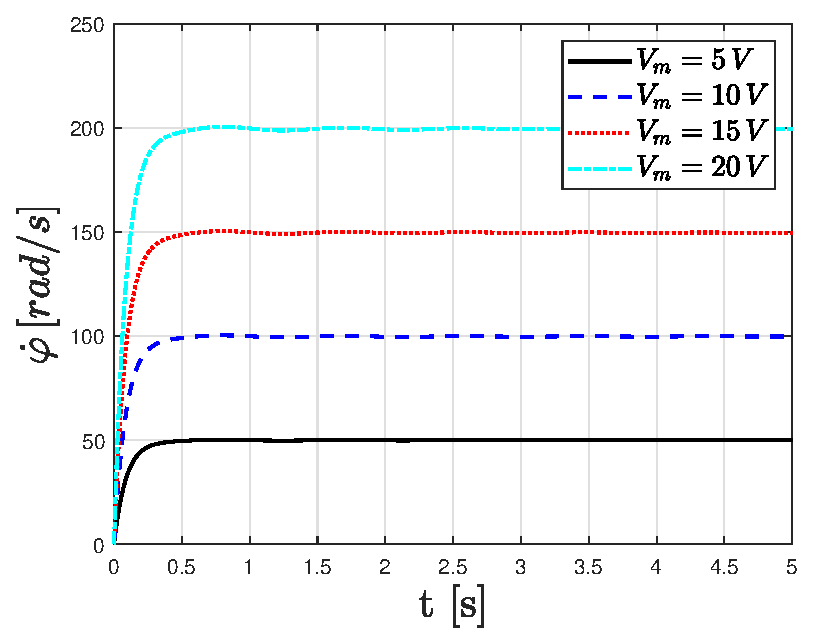
\includegraphics[width=\linewidth]{plot_data/parameter/fig/Vm_sprung/phi_punkt.eps}
        \caption{Schwungrad Geschwindikeit}
        \label{fig:Vm_sprung_phi_punkt}
    \end{subfigure}
    \begin{subfigure}[b]{0.49 \linewidth}
        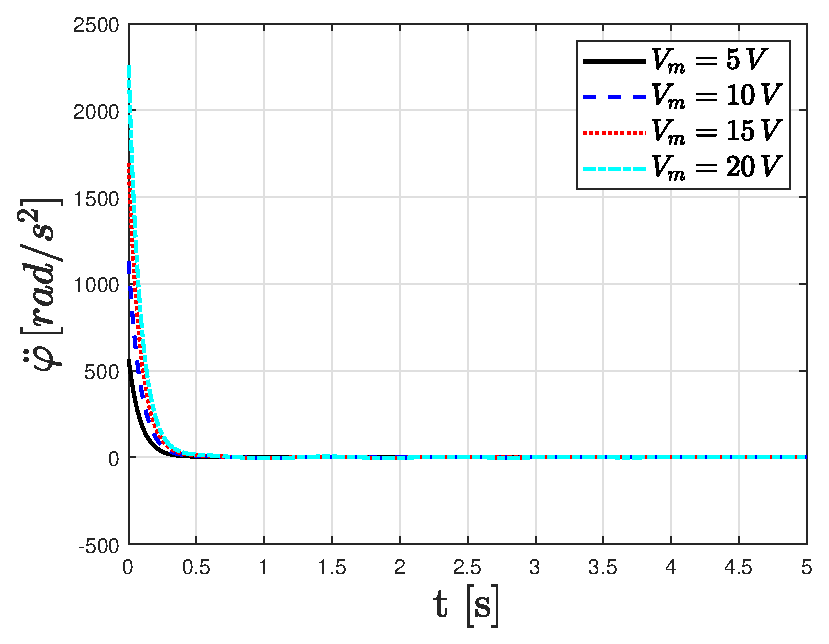
\includegraphics[width=\linewidth]{plot_data/parameter/fig/Vm_sprung/phi_punkt_punkt.eps}
        \caption{Schwungrad Beschleunigung}
        \label{fig:Vm_sprung_phi_punkt_punkt}
    \end{subfigure}
    \begin{subfigure}[b]{0.49 \linewidth}
        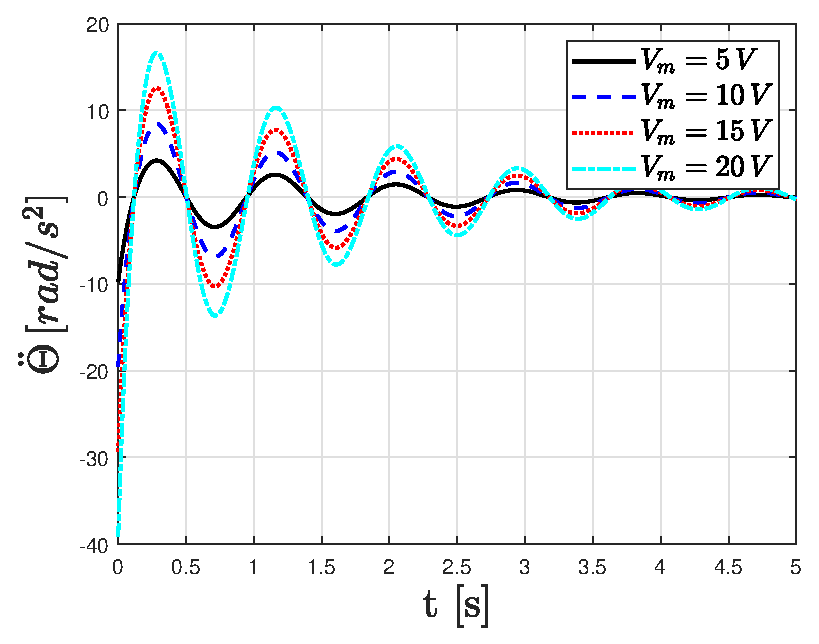
\includegraphics[width=\linewidth]{plot_data/parameter/fig/Vm_sprung/theta_punkt_punkt.eps}
        \caption{Pendel Beschleunigung}
        \label{fig:Vm_sprung_theta_punkt_punkt}
    \end{subfigure}
    \begin{subfigure}[b]{0.49\linewidth}
        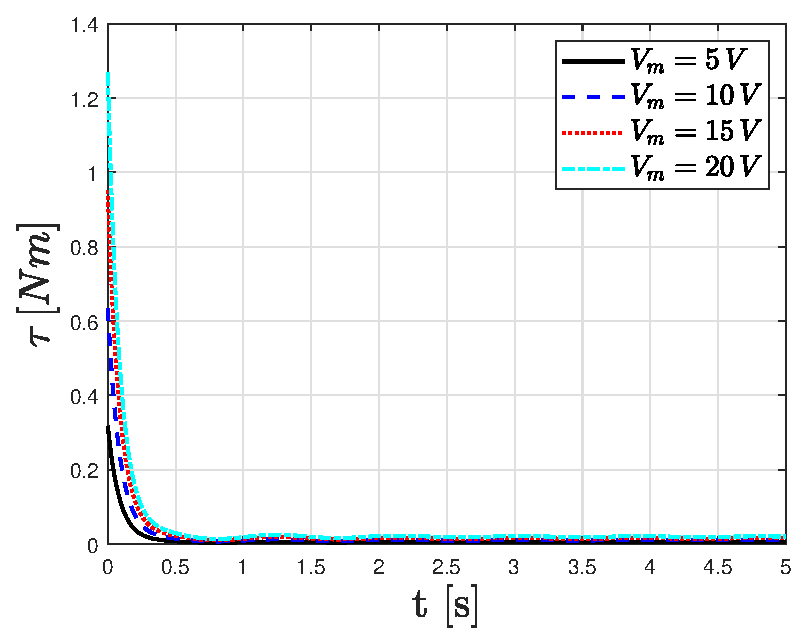
\includegraphics[width=\linewidth]{plot_data/parameter/fig/Vm_sprung/tau.eps}
        \caption{Motor Moment}
        \label{fig:Vm_sprung_tau}
    \end{subfigure}
    \begin{subfigure}[b]{0.49\linewidth}
        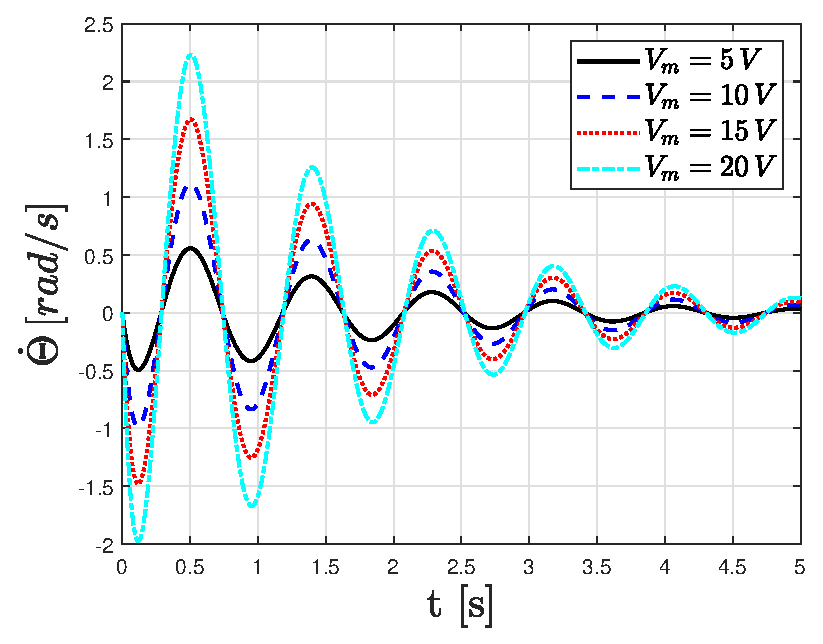
\includegraphics[width=\linewidth]{plot_data/parameter/fig/Vm_sprung/theta_punkt.eps}
        \caption{Pendel Geschwindigkeit}
        \label{fig:Vm_sprung_theta_punkt}      
    \end{subfigure}
    \begin{subfigure}[b]{0.49\linewidth}
        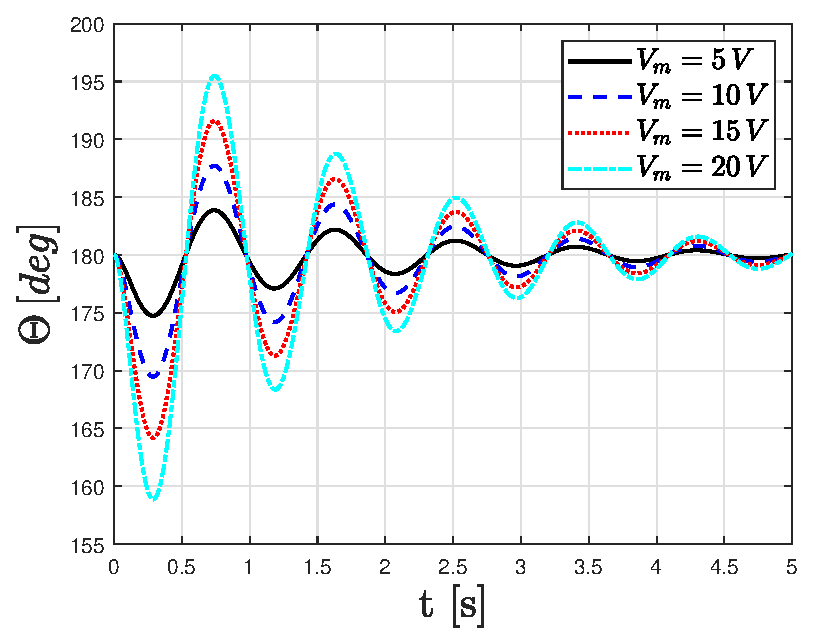
\includegraphics[width=\linewidth]{plot_data/parameter/fig/Vm_sprung/theta.eps}
        \caption{Pendel Winkel}
        \label{fig:Vm_sprung_theta}
    \end{subfigure}
        \caption{Modellantwort auf Eingangssprung der Motorspannung}
\end{wrapfigure}
In Abb.\,\ref{fig:Vm_sprung_phi_punkt} ist zu erkennen, dass der stabile Zustand der Endgeschwindigkeit des Schwungrades ungefähr zur selber Zeit ($t=\SI{0.5}{\s}$) erreicht wird.
Die dabei erreichte Endgeschwindigkeit ist direkt abhängig von der angelegten Motorsspannung $V_m$.\\
Das Maximum des Motormomentes hängt dabei ebenso von der Höhe der angelegten Motorsspannung $V_m$ ab (Abb. \ref{fig:Vm_sprung_tau}).
Das Moment erzeugt dabei eine Beschleunigung des Schwungrades (Abb. \ref{fig:Vm_sprung_phi_punkt_punkt}), die ebenso durch das Moment in Abhängigkeit zur Höhe des angelegten Motorstrommes steht.

Das Pendel wird durch das Moment in Bewegung versetzt und schwingt in Eigenfrequnz (Abb. \ref{fig:Vm_sprung_theta}). 
Die Amplitude der Pendelbewegung ist dabei abhängig von der Höhe der angelegten Motorsspannung $V_m$.

Die Pendelgeschwindigkeit (Abb. \ref{fig:Vm_sprung_theta_punkt}) hat ihren Nulldurchgang beim maximaller Amplitude des Pendelwinkels (Abb. \ref{fig:Vm_sprung_tau}), wobei die maximale Pendelgeschwindigkeit bei $\tau=\SI{180}{\degree}$ erreicht wird.

Nach erreichen der Endgeschwindigkeit des Schwungrades, geht die Beschleunigung gegen Null und das Motormomente gleicht dem Reibungsmoment (Abb. \ref{fig:Vm_sprung_tau}).
Das Pendel ist ab diesen Moment nur noch durch die Gravitation beeinfluss und schwing solange bis es in Ruheposition zurückkehrt.

\subsection*{Einfluss der Länge des Pendels zum Massezentrum des Schwungrades (l2)}
Die Länge von der Aufhängung des Pendels bis zum Masseschwerpunkt des Schwungrades ($l2$) ist ein weiterer Parameter er im Folgenden unterscuht wird.
In den Simualtionen (Abb. \ref{fig:l2}) wurde der Parameter $l2$ von $\SI{0.1}{\m}$ bis $\SI{1.5}{\m}$ variiert.
Die Motorspannung wrd dabei auf \SI{10}{\volt} gesetzt und die anderen Parameter werden ebenfals auf die Standardwerte in Tab. \ref{tab:Tabelle1.1} festgelegt.
\pagebreak

\begin{wrapfigure}{l}{.5\textwidth}
    \captionsetup[subfigure]{justification=centering,font=footnotesize}
    \begin{subfigure}[b]{0.49\linewidth}
        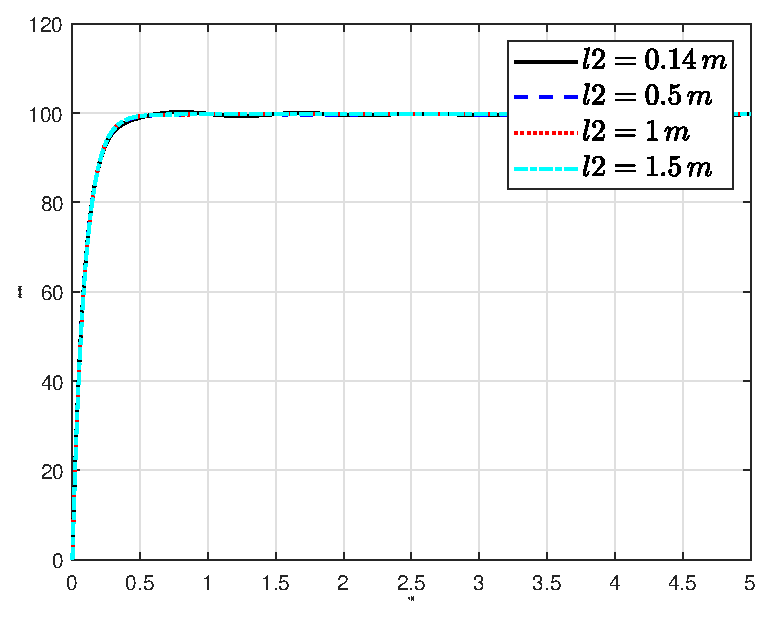
\includegraphics[width=\linewidth]{plot_data/parameter/fig/l2/phi_punkt.eps}
        \caption{Schwungrad Geschwindikeit}
        \label{fig:l2_phi_punkt}
    \end{subfigure}
    \begin{subfigure}[b]{0.49 \linewidth}
        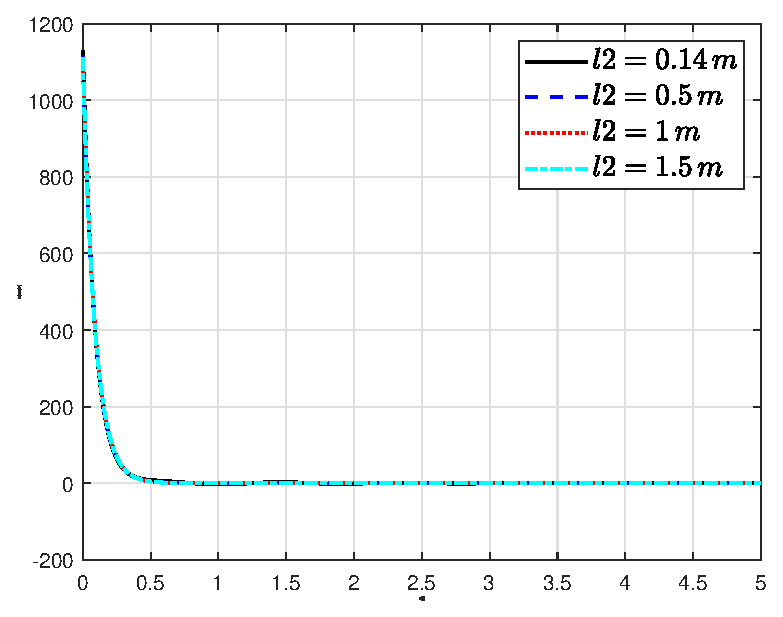
\includegraphics[width=\linewidth]{plot_data/parameter/fig/l2/phi_punkt_punkt.eps}
        \caption{Schwungrad Beschleunigung}
        \label{fig:l2_phi_punkt_punkt}
    \end{subfigure}
    \begin{subfigure}[b]{0.49 \linewidth}
        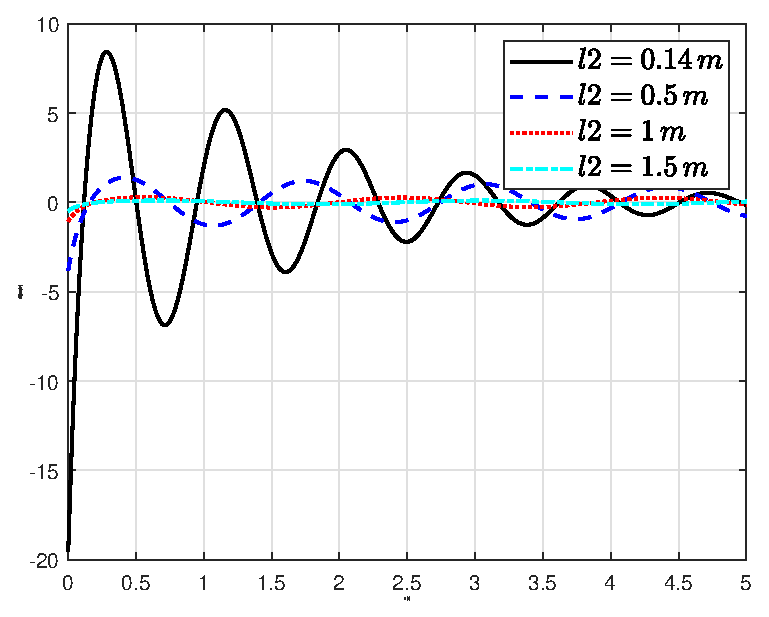
\includegraphics[width=\linewidth]{plot_data/parameter/fig/l2/theta_punkt_punkt.eps}
        \caption{Pendel Beschleunigung}
        \label{fig:l2_theta_punkt_punkt}
    \end{subfigure}
    \begin{subfigure}[b]{0.49\linewidth}
        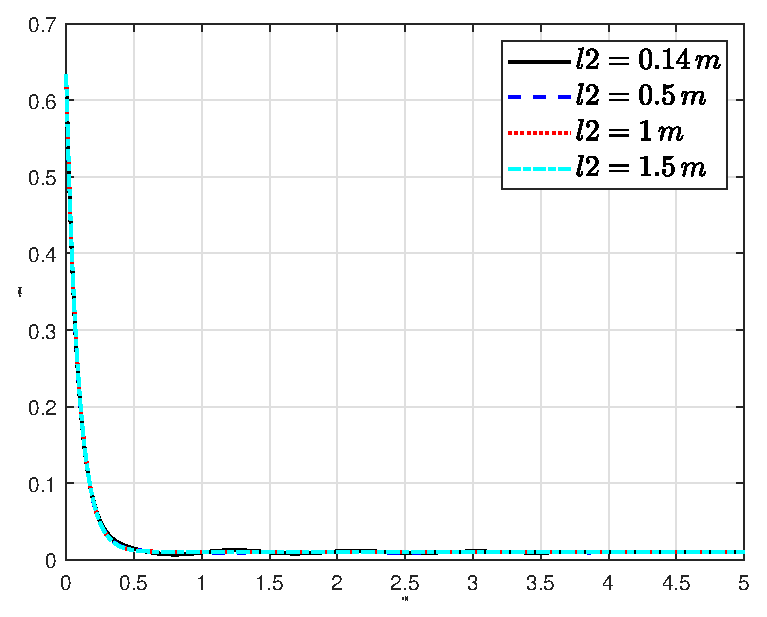
\includegraphics[width=\linewidth]{plot_data/parameter/fig/l2/tau.eps}
        \caption{Motor Moment}
        \label{fig:l2_tau}
    \end{subfigure}
    \begin{subfigure}[b]{0.49\linewidth}
        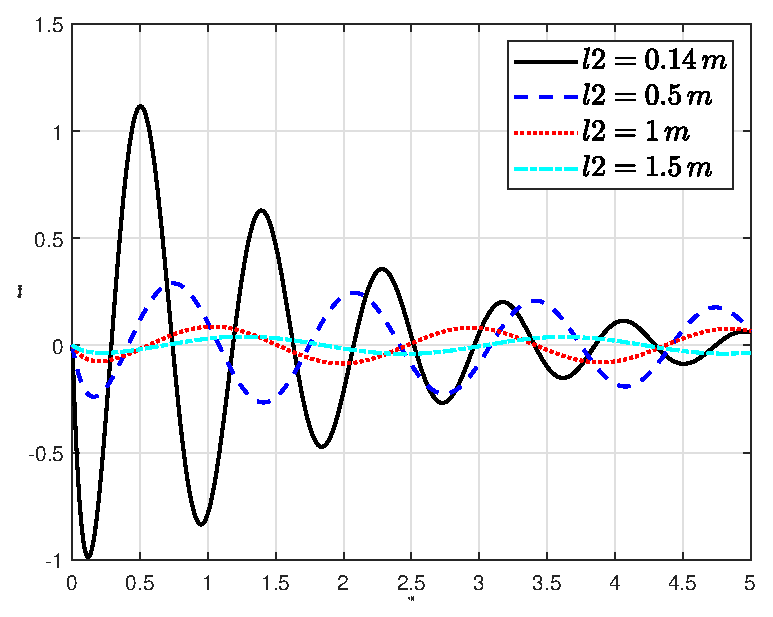
\includegraphics[width=\linewidth]{plot_data/parameter/fig/l2/theta_punkt.eps}
        \caption{Pendel Geschwindigkeit}
        \label{fig:l2_theta_punkt}      
    \end{subfigure}
    \begin{subfigure}[b]{0.49\linewidth}
        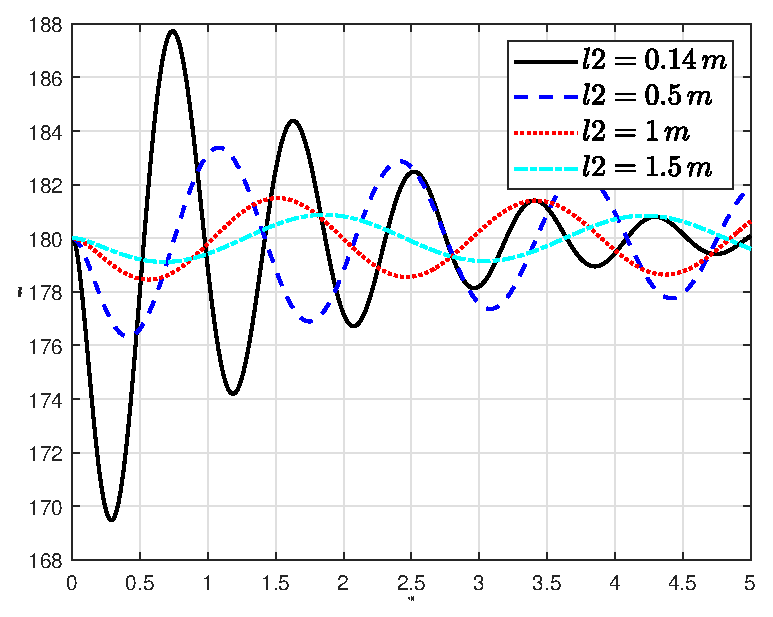
\includegraphics[width=\linewidth]{plot_data/parameter/fig/l2/theta.eps}
        \caption{Pendel Winkel}
        \label{fig:l2_theta}
    \end{subfigure}
        \caption{Modellantwort auf Varianz des Parameters: $l2$}
        \label{fig:l2}
\end{wrapfigure}
Abbildung \ref{fig:l2_phi_punkt}, \ref{fig:l2_phi_punkt}, \ref{fig:l2_tau} zeigen keine Abweichung, was zeigt das der Parameter $l2$ keinen Einfluss auf die Modellgrößen $\dot\varphi,\ddot\varphi,\tau$ hat.
Es ist jdeoch ein Einfluss auf die Parameter $\Theta,\dot\Theta,\ddot\Theta$ (Abb. \ref{fig:l2_theta}\ref{fig:l2_theta_punkt}\ref{fig:l2_theta_punkt_punkt}) zu erkennen. 

Bei kleinerer Länge $l2$ erhöht sich die Amplitude des Winkels $\Theta$ sowie dessen Geschwindigkeit $\dot\Theta$ und Beschleunigung $\ddot\Theta$. 

Ebenso ist zu erkennen das sich dei Eigenfrequenz, mit der das Pendel Schwing verändert.
Je größer die Länge $l2$ ist, desto größeres Moment musss aufgebracht werden um die gleiche Winkelauslenkung $\Theta$ zu erreichen. 
Daraus folgt, dass größere Pendelängen die Winkelantwort des Modelles verschlechtern. 

\subsection*{Einfluss des Trägheitsmoments des Schwungrads (J2)}
Der Einfluss des Trägheitsmoments des Schwungrades ($J2$), auf die Modellparameter wird in den Simulationen (Abb. \ref{fig:j2}) untersucht. 
Der Parameter $J2$ wird dabei von $\SI{0.0005}{\kg\m^2}$ bis $\SI{0.008}{\kg\m^2}$ variiert.
Die Motorspannung wrd dabei auf \SI{10}{\volt} gesetzt und die anderen Parameter werden ebenfals auf die Standardwerte in Tab. \ref{tab:Tabelle1.1} festgelegt.\\
\pagebreak

\begin{wrapfigure}{l}{0.5\textwidth}
    \captionsetup[subfigure]{justification=centering,font=footnotesize}
    \begin{subfigure}[b]{0.49\linewidth}
        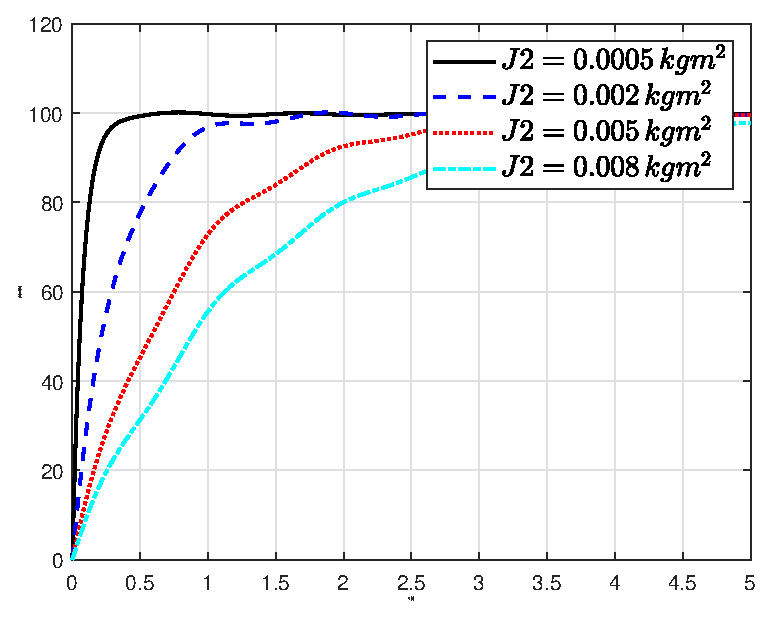
\includegraphics[width=\linewidth]{plot_data/parameter/fig/j2/phi_punkt.eps}
        \caption{Schwungrad Geschwindikeit}
        \label{fig:j2_phi_punkt}
    \end{subfigure}
    \begin{subfigure}[b]{0.49 \linewidth}
        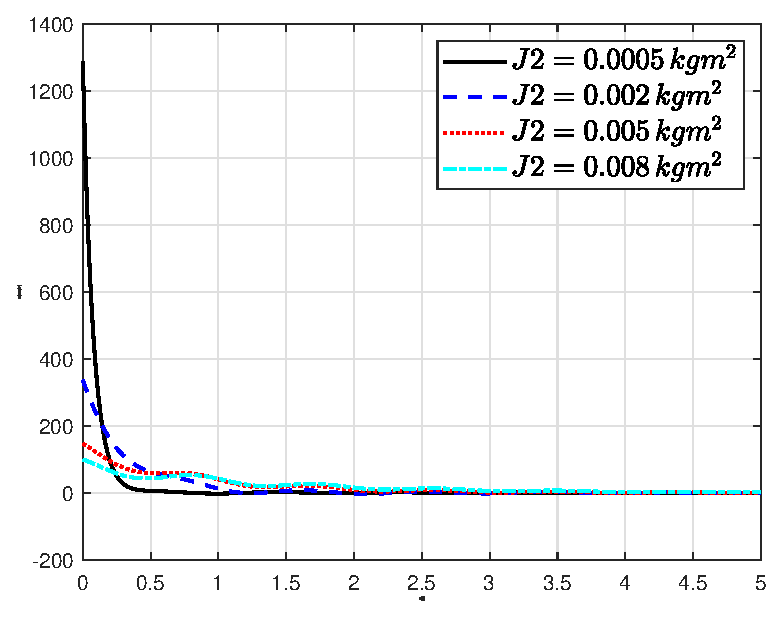
\includegraphics[width=\linewidth]{plot_data/parameter/fig/j2/phi_punkt_punkt.eps}
        \caption{Schwungrad Beschleunigung}
        \label{fig:j2_phi_punkt_punkt}
    \end{subfigure}
    \begin{subfigure}[b]{0.49 \linewidth}
        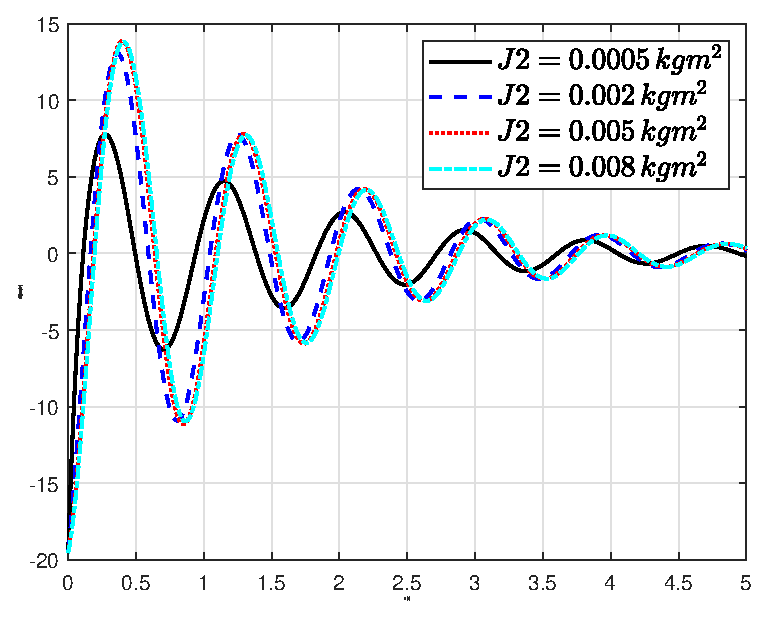
\includegraphics[width=\linewidth]{plot_data/parameter/fig/j2/theta_punkt_punkt.eps}
        \caption{Pendel Beschleunigung}
        \label{fig:j2_theta_punkt_punkt}
    \end{subfigure}
    \begin{subfigure}[b]{0.49\linewidth}
        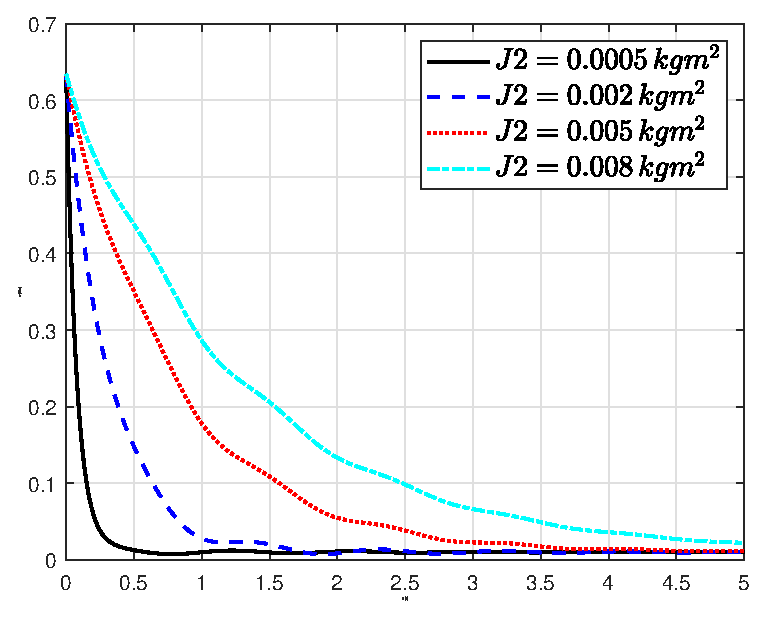
\includegraphics[width=\linewidth]{plot_data/parameter/fig/j2/tau.eps}
        \caption{Motor Moment}
        \label{fig:j2_tau}
    \end{subfigure}
    \begin{subfigure}[b]{0.49\linewidth}
        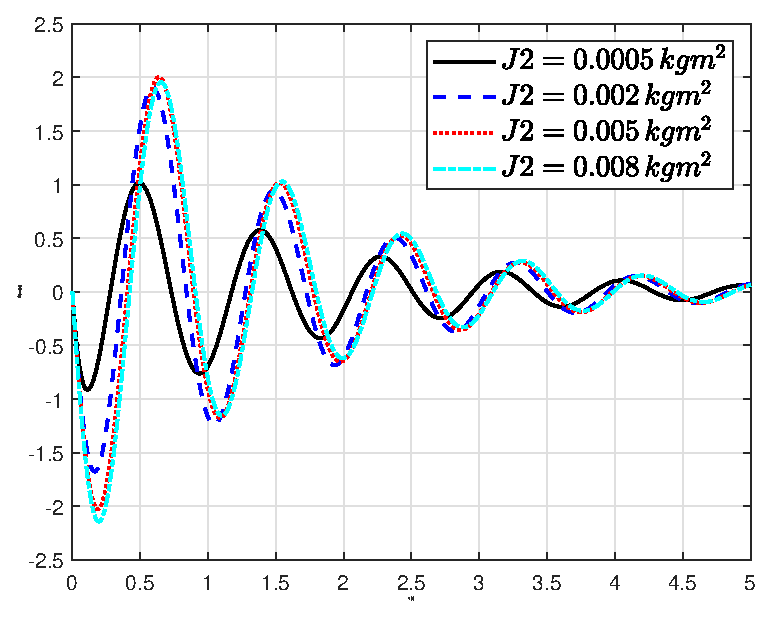
\includegraphics[width=\linewidth]{plot_data/parameter/fig/j2/theta_punkt.eps}
        \caption{Pendel Geschwindigkeit}
        \label{fig:j2_theta_punkt}      
    \end{subfigure}
    \begin{subfigure}[b]{0.49\linewidth}
        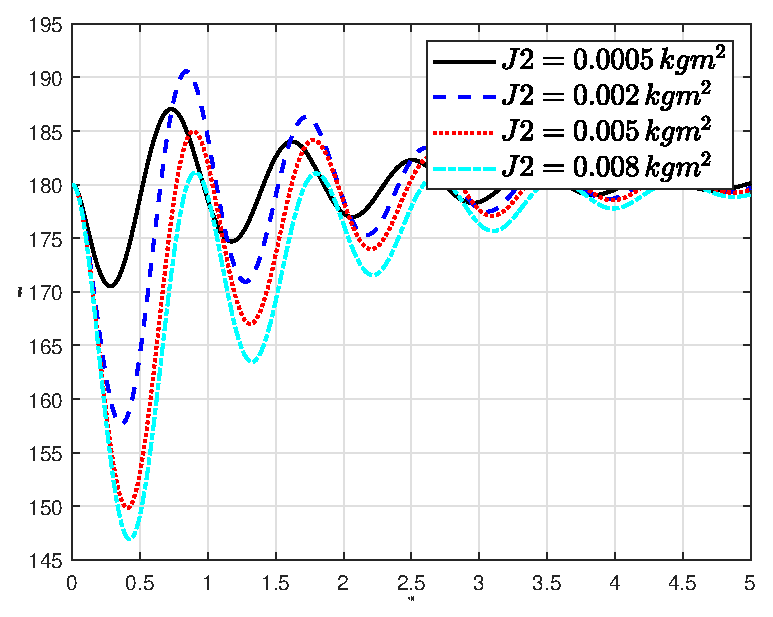
\includegraphics[width=\linewidth]{plot_data/parameter/fig/j2/theta.eps}
        \caption{Pendel Winkel}
        \label{fig:j2_theta}
    \end{subfigure}
        \caption{Modellantwort auf Varianz des Parameters: $J2$}
        \label{fig:j2}
\end{wrapfigure}
Die stationäre Endgeschwindigkeit des Schwungrades, wird durch den Parameter $J2$ stark beinflusst (Abb. \ref{fig:j2_phi_punkt}). 
Bei erhöhter Trägheit des Schwungrades erhöht sich die Anstiegszeit, bis ein eingeschwungener Zustand erreicht wird.
Der Wert konvergiert allerdings bei allen Werten von $J2$ gegen die gleiche Endgeschwindigkeit.\\

Die Beschleunigung des Schwungrades wird ebenfalls stark beinflusst (Abb. \ref{fig:j2_phi_punkt_punkt}).
Hierbei ist zu erkennen, dass ein erhöhtes Trägheitsmoment die maximale Beschleunigung bei $t\approx\SI{0}{\s}$ verringert. 
Ebenso wird der stationäre Zustand später erreicht und mit weiterer Erhöhung des Parameters ist ein Schwingen der Beschleunigung zu erkennen.\\
   
Das maximale Motormoment (Abb. \ref{fig:j2_tau}) ist bei allen Werten von $J2$ gleich, benötigt aber bei größeren Werten von $J2$ länger um den stationären Zustand zu erreichen.\\
Dadurch dass das Moment bei erhöhten Trägheitsmoment länger anliegt, wird auch eine größere Kraft auf das Pendel ausgeübt(Abb. \ref{fig:j2_theta_punkt_punkt}).\\
In Abb.\ref{fig:j2_theta} ist zu erkennen, dass ein größere Winkelauschlag des Pendels erreicht wurde.\\
Dies ist ebenso der Fall bei der Pendelbeschleunigung (Abb. \ref{fig:j2_theta_punkt_punkt}) und der Pendelgeschwindigkeit (Abb. \ref{fig:j2_theta_punkt}).\\

 Das Trägheitsmoment des Schwungrades $J2$ hat also einen positiven Einfluss auf die Winkelantwort des Modells.\\  
 
 \subsection*{Einfluss der Masse des Schwungrads (M2)}
 Der Einfluss der Masse des Schwungrades ($m2$), auf die Modellparameter wird in den Simulationen (Abb. \ref{fig:m2}) untersucht. 
 Der Parameter $J2$ wird dabei von $\SI{0.01}{\kg}$ bis $\SI{1.5}{\kg}$ variiert.
 Die Motorspannung wrd dabei auf \SI{10}{\volt} gesetzt und die anderen Parameter werden ebenfals auf die Standardwerte in Tab. \ref{tab:Tabelle1.1} festgelegt.\\
 \begin{wrapfigure}{l}{0.5\textwidth}
    \captionsetup[subfigure]{justification=centering,font=footnotesize}
    \begin{subfigure}[b]{0.49\linewidth}
        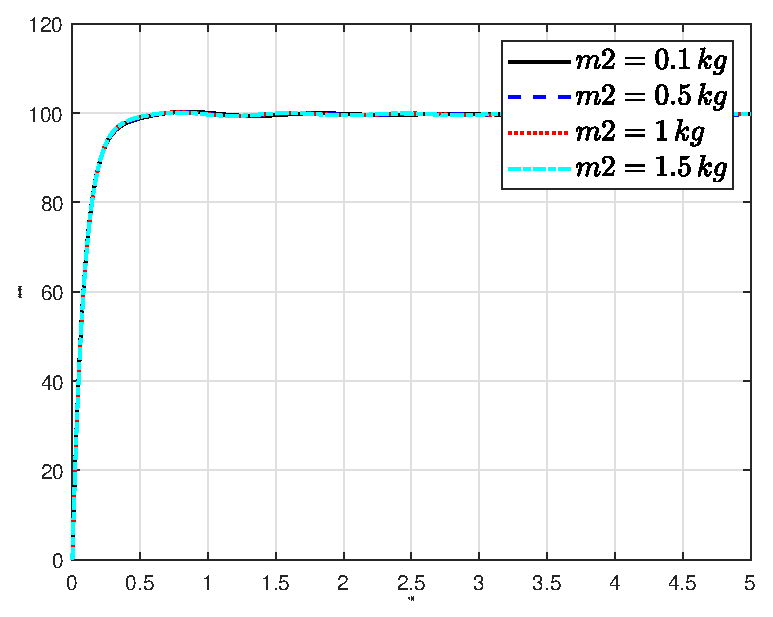
\includegraphics[width=\linewidth]{plot_data/parameter/fig/m2/phi_punkt.eps}
        \caption{Schwungrad Geschwindikeit}
        \label{fig:m2_phi_punkt}
    \end{subfigure}
    \begin{subfigure}[b]{0.49 \linewidth}
        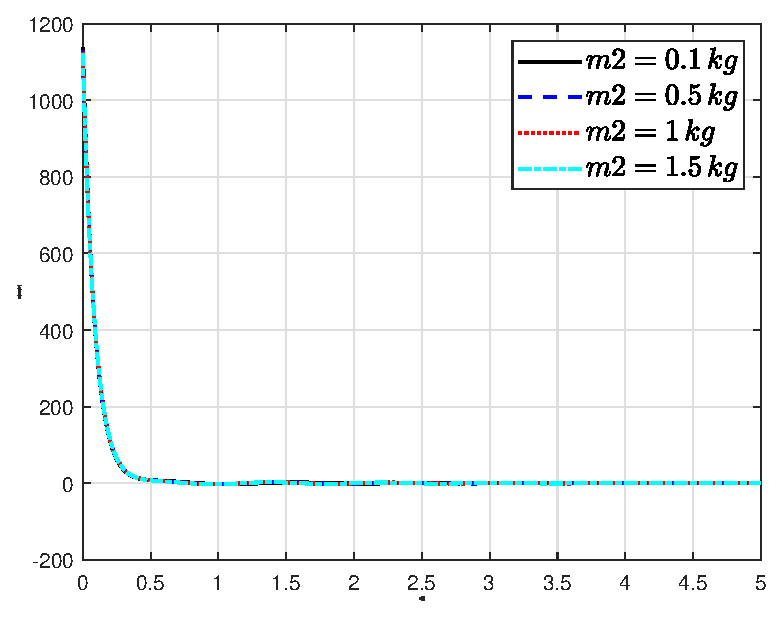
\includegraphics[width=\linewidth]{plot_data/parameter/fig/m2/phi_punkt_punkt.eps}
        \caption{Schwungrad Beschleunigung}
        \label{fig:m2_phi_punkt_punkt}
    \end{subfigure}
    \begin{subfigure}[b]{0.49 \linewidth}
        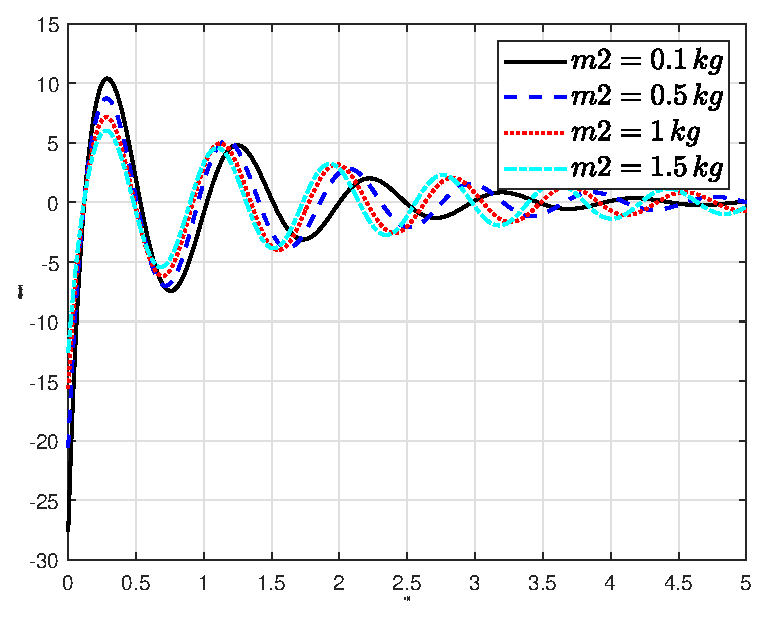
\includegraphics[width=\linewidth]{plot_data/parameter/fig/m2/theta_punkt_punkt.eps}
        \caption{Pendel Beschleunigung}
        \label{fig:m2_theta_punkt_punkt}
    \end{subfigure}
    \begin{subfigure}[b]{0.49\linewidth}
        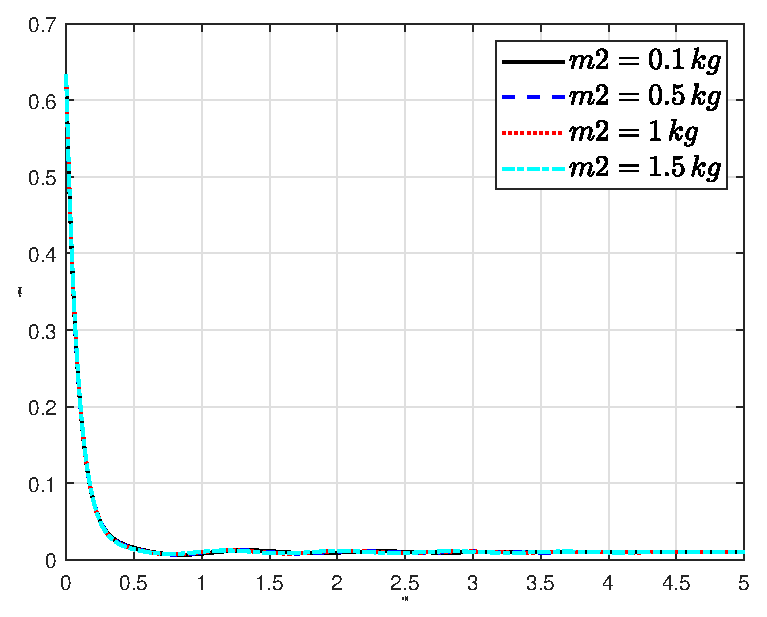
\includegraphics[width=\linewidth]{plot_data/parameter/fig/m2/tau.eps}
        \caption{Motor Moment}
        \label{fig:m2_tau}
    \end{subfigure}
    \begin{subfigure}[b]{0.49\linewidth}
        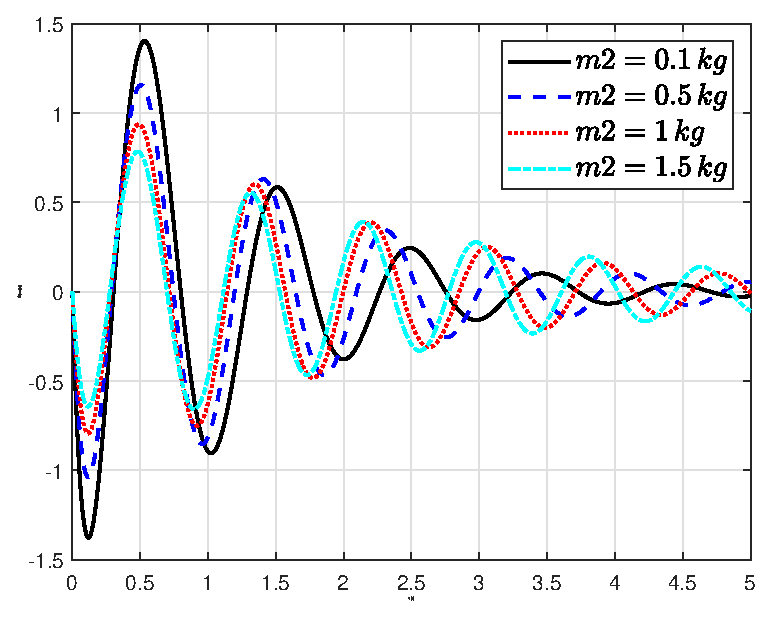
\includegraphics[width=\linewidth]{plot_data/parameter/fig/m2/theta_punkt.eps}
        \caption{Pendel Geschwindigkeit}
        \label{fig:m2_theta_punkt}      
    \end{subfigure}
    \begin{subfigure}[b]{0.49\linewidth}
        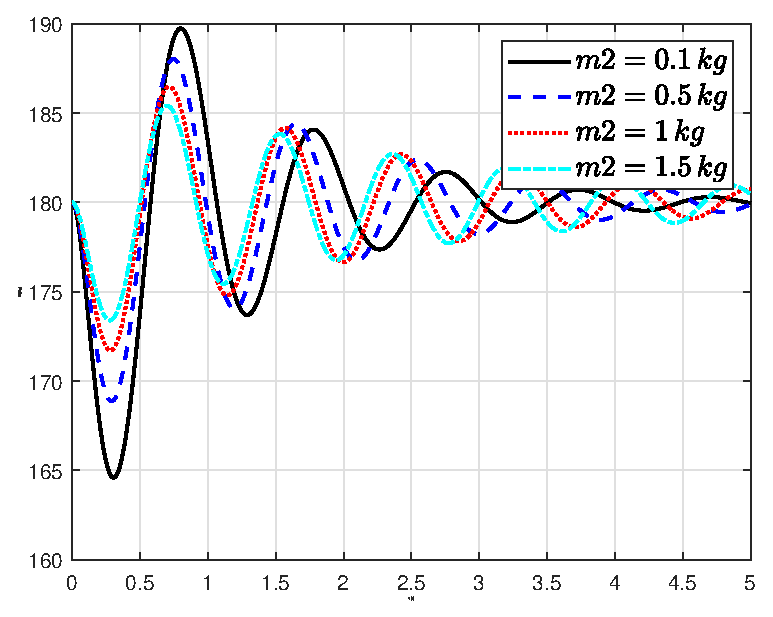
\includegraphics[width=\linewidth]{plot_data/parameter/fig/m2/theta.eps}
        \caption{Pendel Winkel}
        \label{fig:m2_theta}
    \end{subfigure}
        \caption{Modellantwort auf Varianz des Parameters: $M2$}
        \label{fig:m2}
\end{wrapfigure}

In den Simulationen ist zu erkennen das die Schwungradgeschwindigkeit (\ref{fig:m2_phi_punkt}), die Schwungradbeschleunigung (\ref{fig:m2_phi_punkt_punkt}) und das Motormoment (\ref{fig:m2_tau}) durch den Parameter $m2$ nicht beeinflusst werden.\\
Die Masse des Schwungrads hat also auf die gehalten Größen keinen Einfluss.\\

Der Winkel des Pendels (Abb. \ref{fig:m2_theta}) verrignert sich mit erhöhung der Masse $m2$. 
Dies ist auch bei der Pendelgeschwindigkeit (Abb. \ref{fig:m2_theta_punkt}) und der Pendelbeschleunigung (Abb. \ref{fig:m2_theta_punkt_punkt}) zu erkennen.\\
Dies liegt an der, durch die zusätzliche Masse, erhöhten Gewichtskraft, die auf das Pendel wirkt.\\
Ebenso wird die Dämpfung der Schwingung verändert und die Schwingungsdauer verlängert sich.\\

Die erhöhung des Parameters $m2$ trägt also zu einer Verschlechterung der Modellantwort bei.\\



